\documentclass[11pt]{article}
\usepackage[margin=1in]{geometry}
\usepackage{graphicx}
\usepackage{booktabs}
\usepackage{longtable}
\usepackage{amsmath}
\usepackage{float}
\usepackage{hyperref}
\setlength{\parskip}{0.6em}
\setlength{\parindent}{0pt}

\title{Official Gameplay-Driven Battery Sizing Report}
\author{Senior Design Data Analysis Repository}
\date{April 7, 2026}

\begin{document}
\maketitle

\section*{Purpose}
This report explains the official battery-sizing workflow in this repository. The final battery answer comes from cleaned gameplay IMU data only. The project specifications are used to bound the gameplay demand during cleaning, not to create a second battery-sizing branch.

The current official workflow uses:
\begin{itemize}
  \item gameplay trimming from the raw phone exports,
  \item in-place interpolation across collision-like spikes,
  \item acceleration clipping at 2.85 \(\mathrm{m/s^2}\),
  \item surrogate speed capping at 4.91744 \(\mathrm{m/s}\) (11.00 mph),
  \item yaw-aware wheel and motor dynamics,
  \item battery sizing across 24, 36, 48, 60, 72 V and the configured chemistries.
\end{itemize}

\begin{figure}[H]
  \centering
  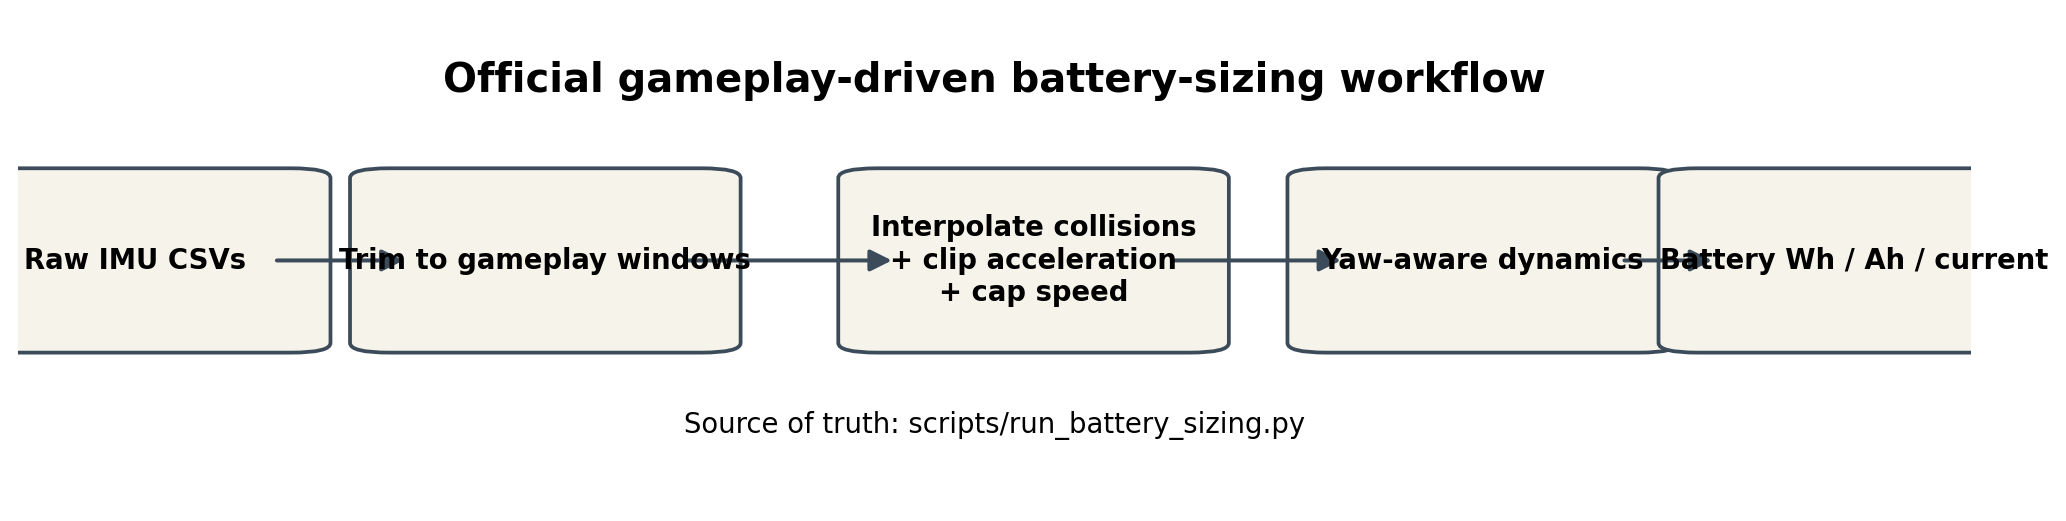
\includegraphics[width=\linewidth]{figures/workflow_diagram.png}
  \caption{Official gameplay-driven battery-sizing workflow used in this repository.}
\end{figure}

\section{Data Provenance}
Two cleaned gameplay sessions are used. Game 1 is the higher-energy session at 230.85 Wh. Game 2 integrates to 192.43 Wh. The manual trimming step removes 53,029 rows from Game 1 and 7,952 rows from Game 2 before the signal-cleaning stage begins.

\begin{tabular}{lllllll}
\toprule
Game & Keep Start (min) & Keep End (min) & Removed Windows & Raw Rows & Cleaned Rows & Rows Removed \\
\midrule
Game1CharlesPhone & 4.0 & 57.5 & 14.5-18.5 min & 350,582 & 297,553 & 53,029 \\
Game2CharlesPhone & 1.0 & 38.4 & None & 232,766 & 224,814 & 7,952 \\
\bottomrule
\end{tabular}


\begin{figure}[H]
  \centering
  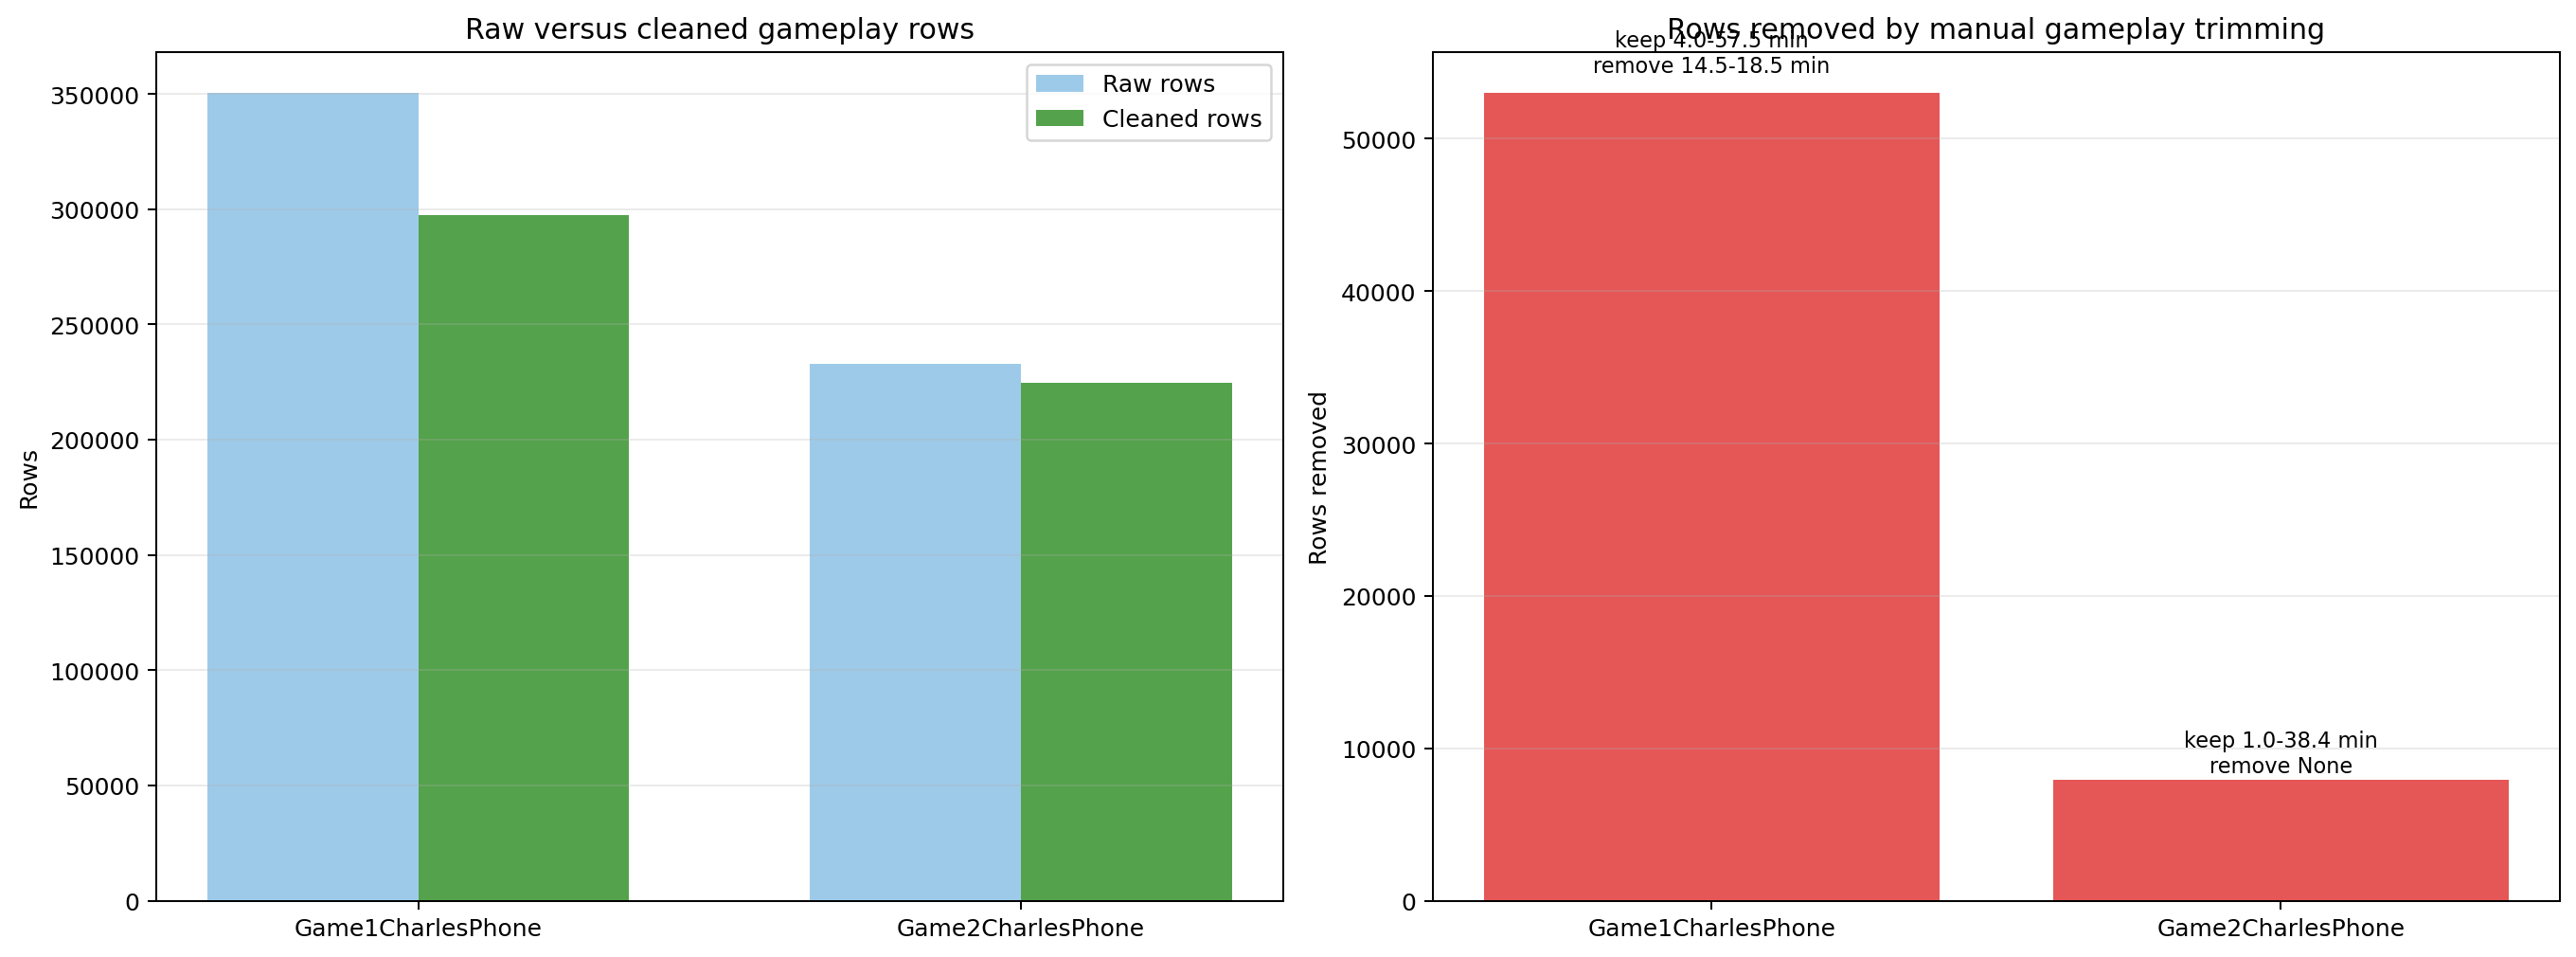
\includegraphics[width=\linewidth]{figures/data_provenance.png}
  \caption{Raw versus cleaned gameplay rows after the repository's trim windows are applied.}
\end{figure}

\section{Signal Cleaning Math}
The phone exports provide user acceleration, gravity, and motion-rotation channels. The repository converts those into a bounded planar propulsion signal.

\textbf{Unit conversion}
\begin{equation}
a_{\mathrm{user},m/s^2} = a_{\mathrm{user},g} \times 9.80665
\end{equation}

\textbf{Planar projection after gravity alignment}
\begin{equation}
\mathbf{a}_{\mathrm{planar}} = \mathbf{a}_{\mathrm{aligned}} - \left(\mathbf{a}_{\mathrm{aligned}} \cdot \hat{g}\right)\hat{g}
\end{equation}

\textbf{Collision detection and interpolation}
Samples are marked when either planar acceleration magnitude or planar jerk exceeds the official thresholds:
\begin{equation}
\|\mathbf{a}_{\mathrm{planar}}\| \ge 25
\quad \text{or} \quad
\left\|\frac{d\mathbf{a}_{\mathrm{planar}}}{dt}\right\| \ge 120
\end{equation}
Those windows are padded by 0.35 s and linearly interpolated in place.

\textbf{Filtering and clipping}
Each planar axis is winsorized at the 99.5th percentile, low-pass filtered, detrended with an 8.0 s rolling median, and clipped to:
\begin{equation}
\|\mathbf{a}_{\mathrm{final}}\| \le 2.85\,\mathrm{m/s^2}
\end{equation}

\textbf{Surrogate speed integration}
The planar acceleration is integrated to a surrogate speed state with zero-velocity resets during stationary periods and a hard cap:
\begin{equation}
\|\mathbf{v}\| \le 4.91744\,\mathrm{m/s}
\end{equation}

\begin{figure}[H]
  \centering
  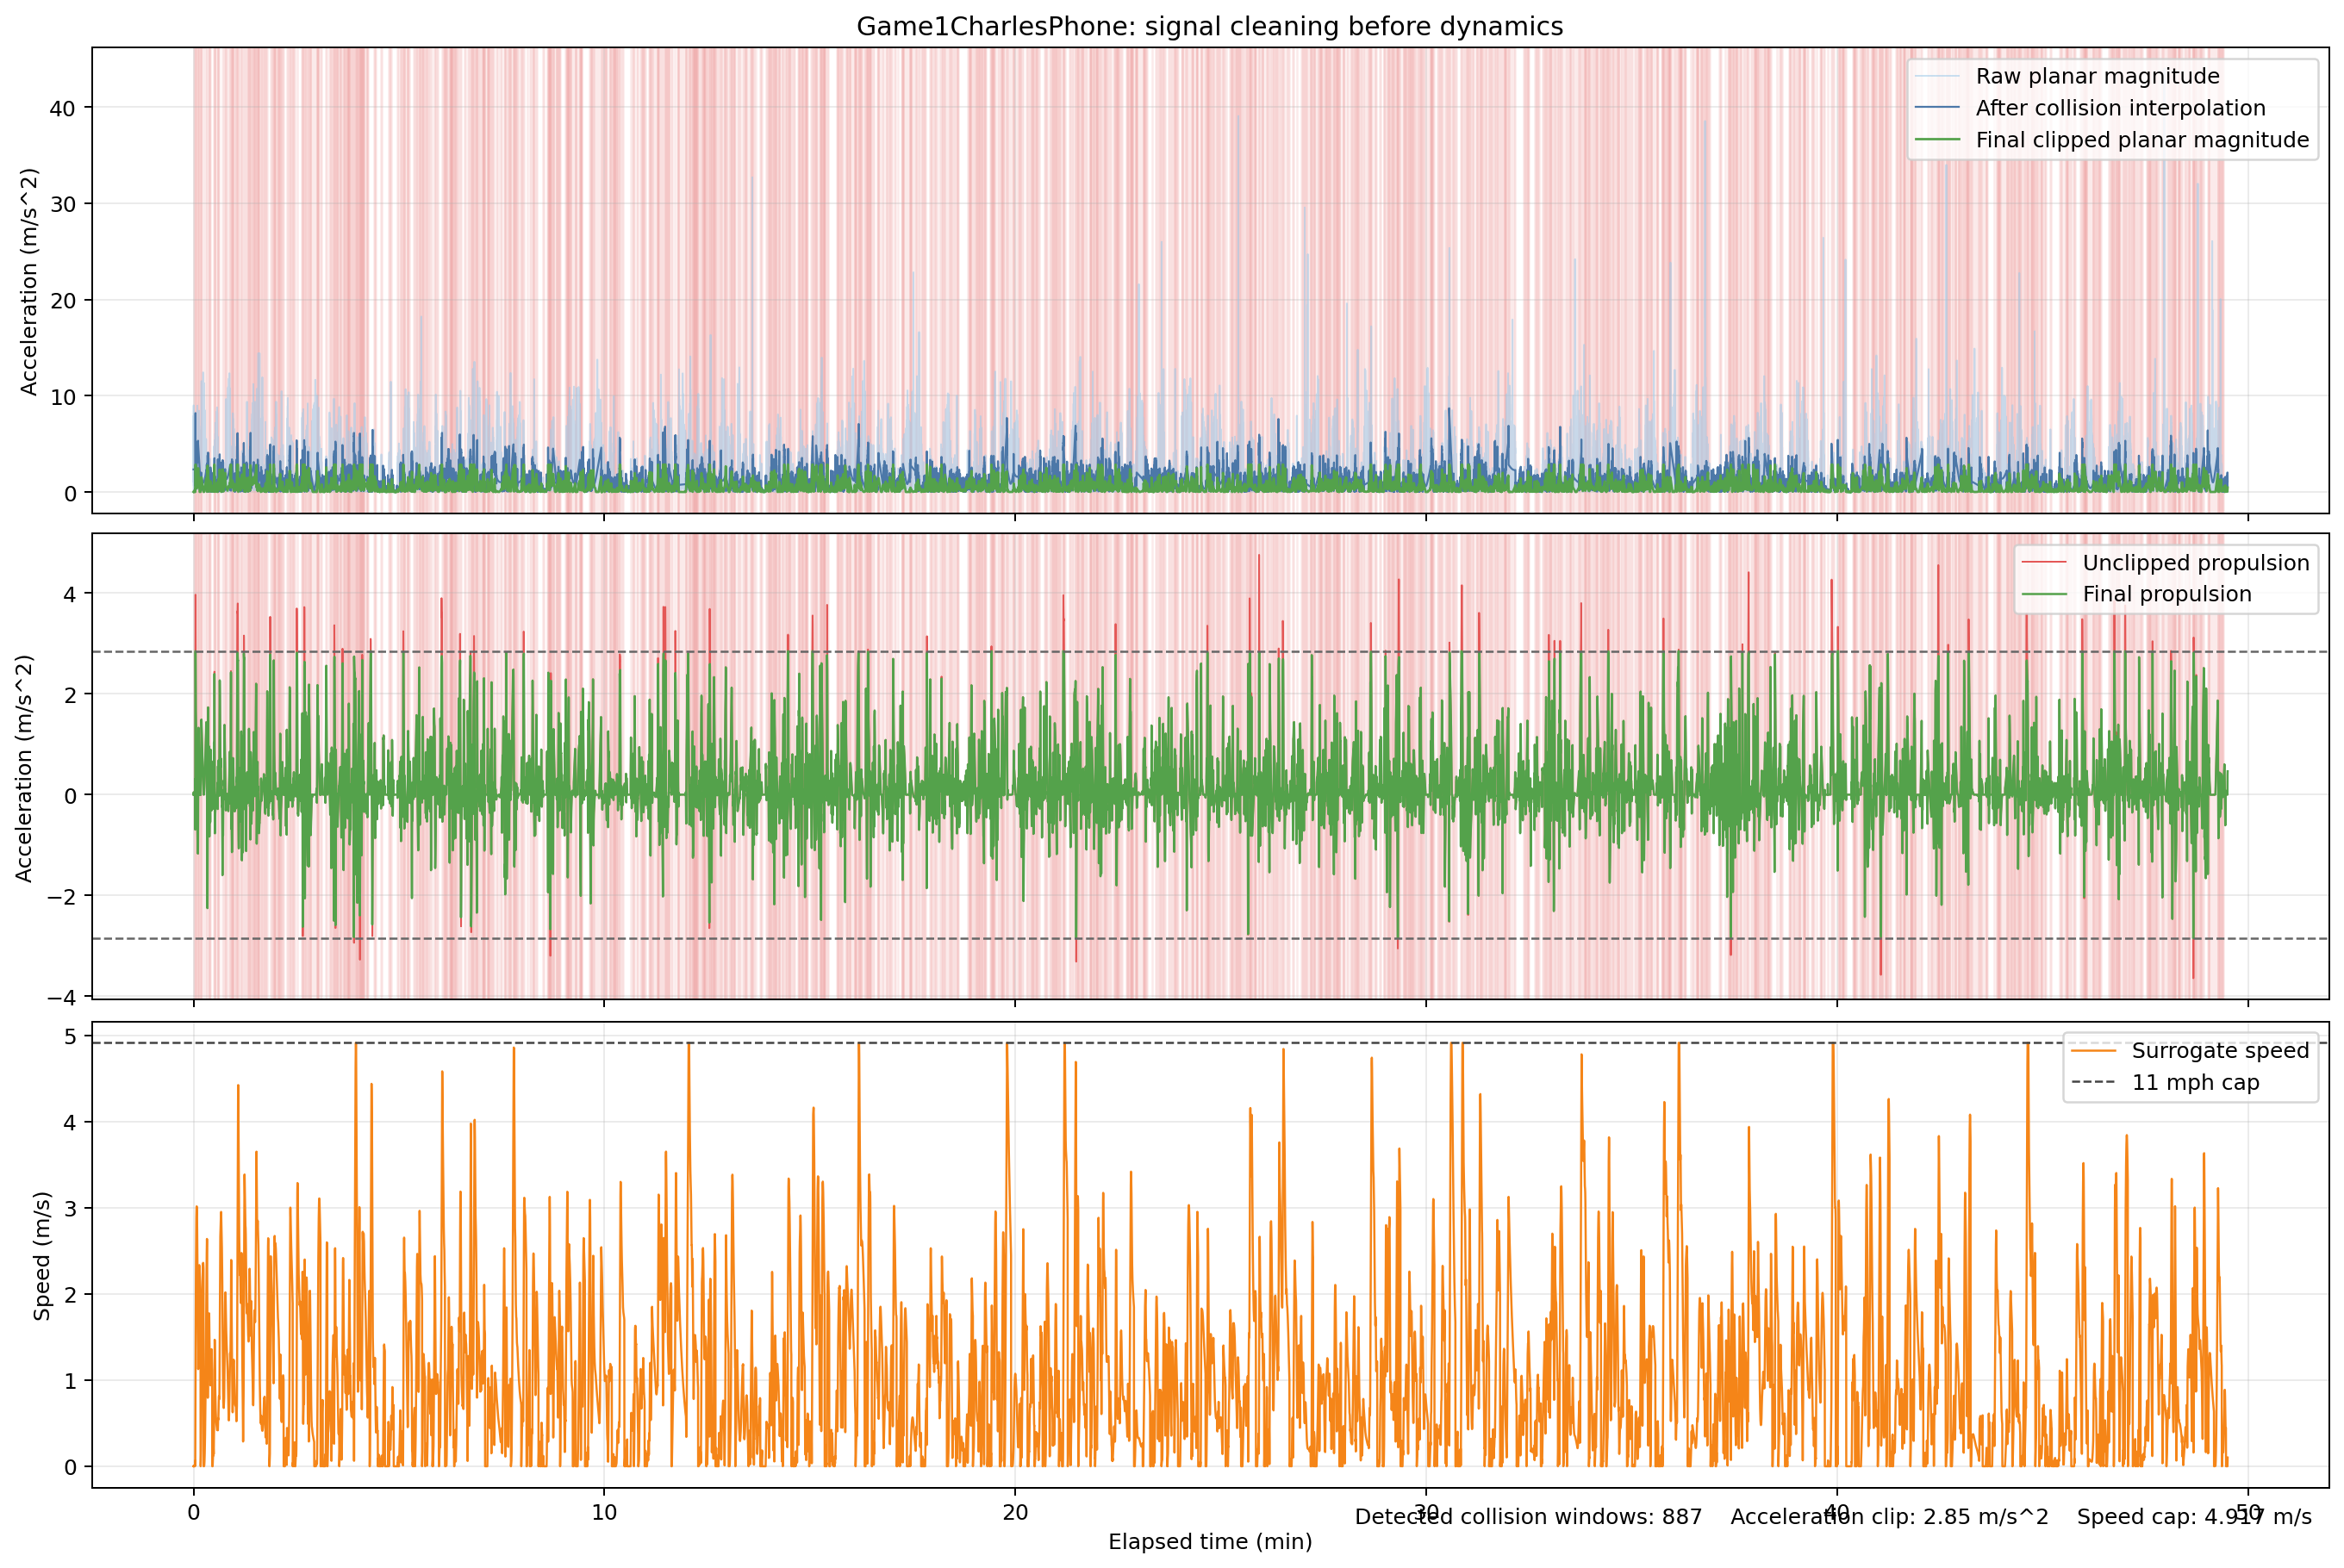
\includegraphics[width=\linewidth]{figures/signal_cleaning.png}
  \caption{How Game 1 is cleaned before the battery model is applied.}
\end{figure}

\section{Dynamics And Battery Math}
With the cleaned gameplay demand in hand, the repository computes wheel load, motor load, and battery load.

The current official workflow fixes total system mass at 105 kg. That means the cleaned gameplay energy is the same across voltages and chemistries. Voltage changes pack current and required amp-hours. Chemistry changes usable fraction, nominal energy, mass, and C-rate checks.

The main force terms are:
\begin{align}
F_{\mathrm{roll}} &= c_{rr} m g \cos(\theta) \\
F_{\mathrm{aero}} &= \frac{1}{2} \rho C_dA v^2 \\
F_{\mathrm{grade}} &= m g \sin(\theta)
\end{align}

For turning, the left and right wheel speeds are:
\begin{align}
v_L &= v - \frac{b}{2}\omega \\
v_R &= v + \frac{b}{2}\omega
\end{align}
with yaw torque:
\begin{equation}
\tau_{\mathrm{yaw}} = I_{\mathrm{yaw}}\alpha_{\mathrm{yaw}}
\end{equation}

Wheel torque, motor torque, and current are:
\begin{align}
\tau_{\mathrm{wheel}} &= rF + I_{\mathrm{wheel}}\frac{a_{\mathrm{wheel}}}{r} \\
\tau_{\mathrm{motor}} &= \frac{\tau_{\mathrm{wheel,per\ motor}}}{G\eta_{gear}} \\
I_{\mathrm{motor}} &= \frac{\tau_{\mathrm{motor}}}{K_t}
\end{align}

No regenerative braking is credited. Battery power is:
\begin{equation}
P_{\mathrm{battery}} =
\begin{cases}
\dfrac{P_{\mathrm{wheel}}}{\eta_{drive}} + P_{\mathrm{aux}}, & P_{\mathrm{wheel}} > 0 \\
P_{\mathrm{aux}}, & P_{\mathrm{wheel}} \le 0
\end{cases}
\end{equation}

The final battery equations are:
\begin{align}
E_{\mathrm{usable}} &= \sum P_{\mathrm{battery}}\,\Delta t / 3600 \\
E_{\mathrm{nom}} &= E_{\mathrm{usable}} / f_{\mathrm{usable}} \\
C_{\mathrm{nom}} &= E_{\mathrm{nom}} / V_{pack} \\
m_{\mathrm{battery}} &= E_{\mathrm{nom}} / e_{\mathrm{specific}}
\end{align}

\section{Worked Example: Game 1 at 48 V with NMC}
This report uses the hardest gameplay session and the common 48 V design point as the worked example.

\begin{tabular}{lll}
\toprule
Quantity & Value & Unit \\
\midrule
Worked example game & Game1CharlesPhone &  \\
Battery chemistry & nmc\_high\_rate &  \\
Pack voltage & 48 & V \\
Cleaned gameplay energy & 230.85 & Wh \\
Battery usable fraction & 0.90 & - \\
Nominal battery energy & 256.50 & Wh \\
Required nominal capacity & 5.344 & Ah \\
Battery mass & 1.603 & kg \\
Peak battery power sample time & 36.14 & min \\
Peak traction force & 323.07 & N \\
Peak wheel torque & 100.48 & N m \\
Peak motor torque & 3.489 & N m \\
Peak motor current & 28.593 & A \\
Peak battery power & 2025.36 & W \\
Peak battery current & 42.195 & A \\
\bottomrule
\end{tabular}


The core battery arithmetic for the worked example is:
\begin{align}
E_{\mathrm{usable}} &= 230.85\,\mathrm{Wh} \\
E_{\mathrm{nom}} &= \frac{230.85}{0.90}
= 256.50\,\mathrm{Wh} \\
C_{\mathrm{nom}} &= \frac{256.50}{48}
= 5.344\,\mathrm{Ah} \\
m_{\mathrm{battery}} &= \frac{256.50}{160}
= 1.603\,\mathrm{kg}
\end{align}

The peak-power sample gives:
\begin{equation}
I_{\mathrm{battery,peak}} = \frac{2025.36}{48}
= 42.195\,\mathrm{A}
\end{equation}

\begin{figure}[H]
  \centering
  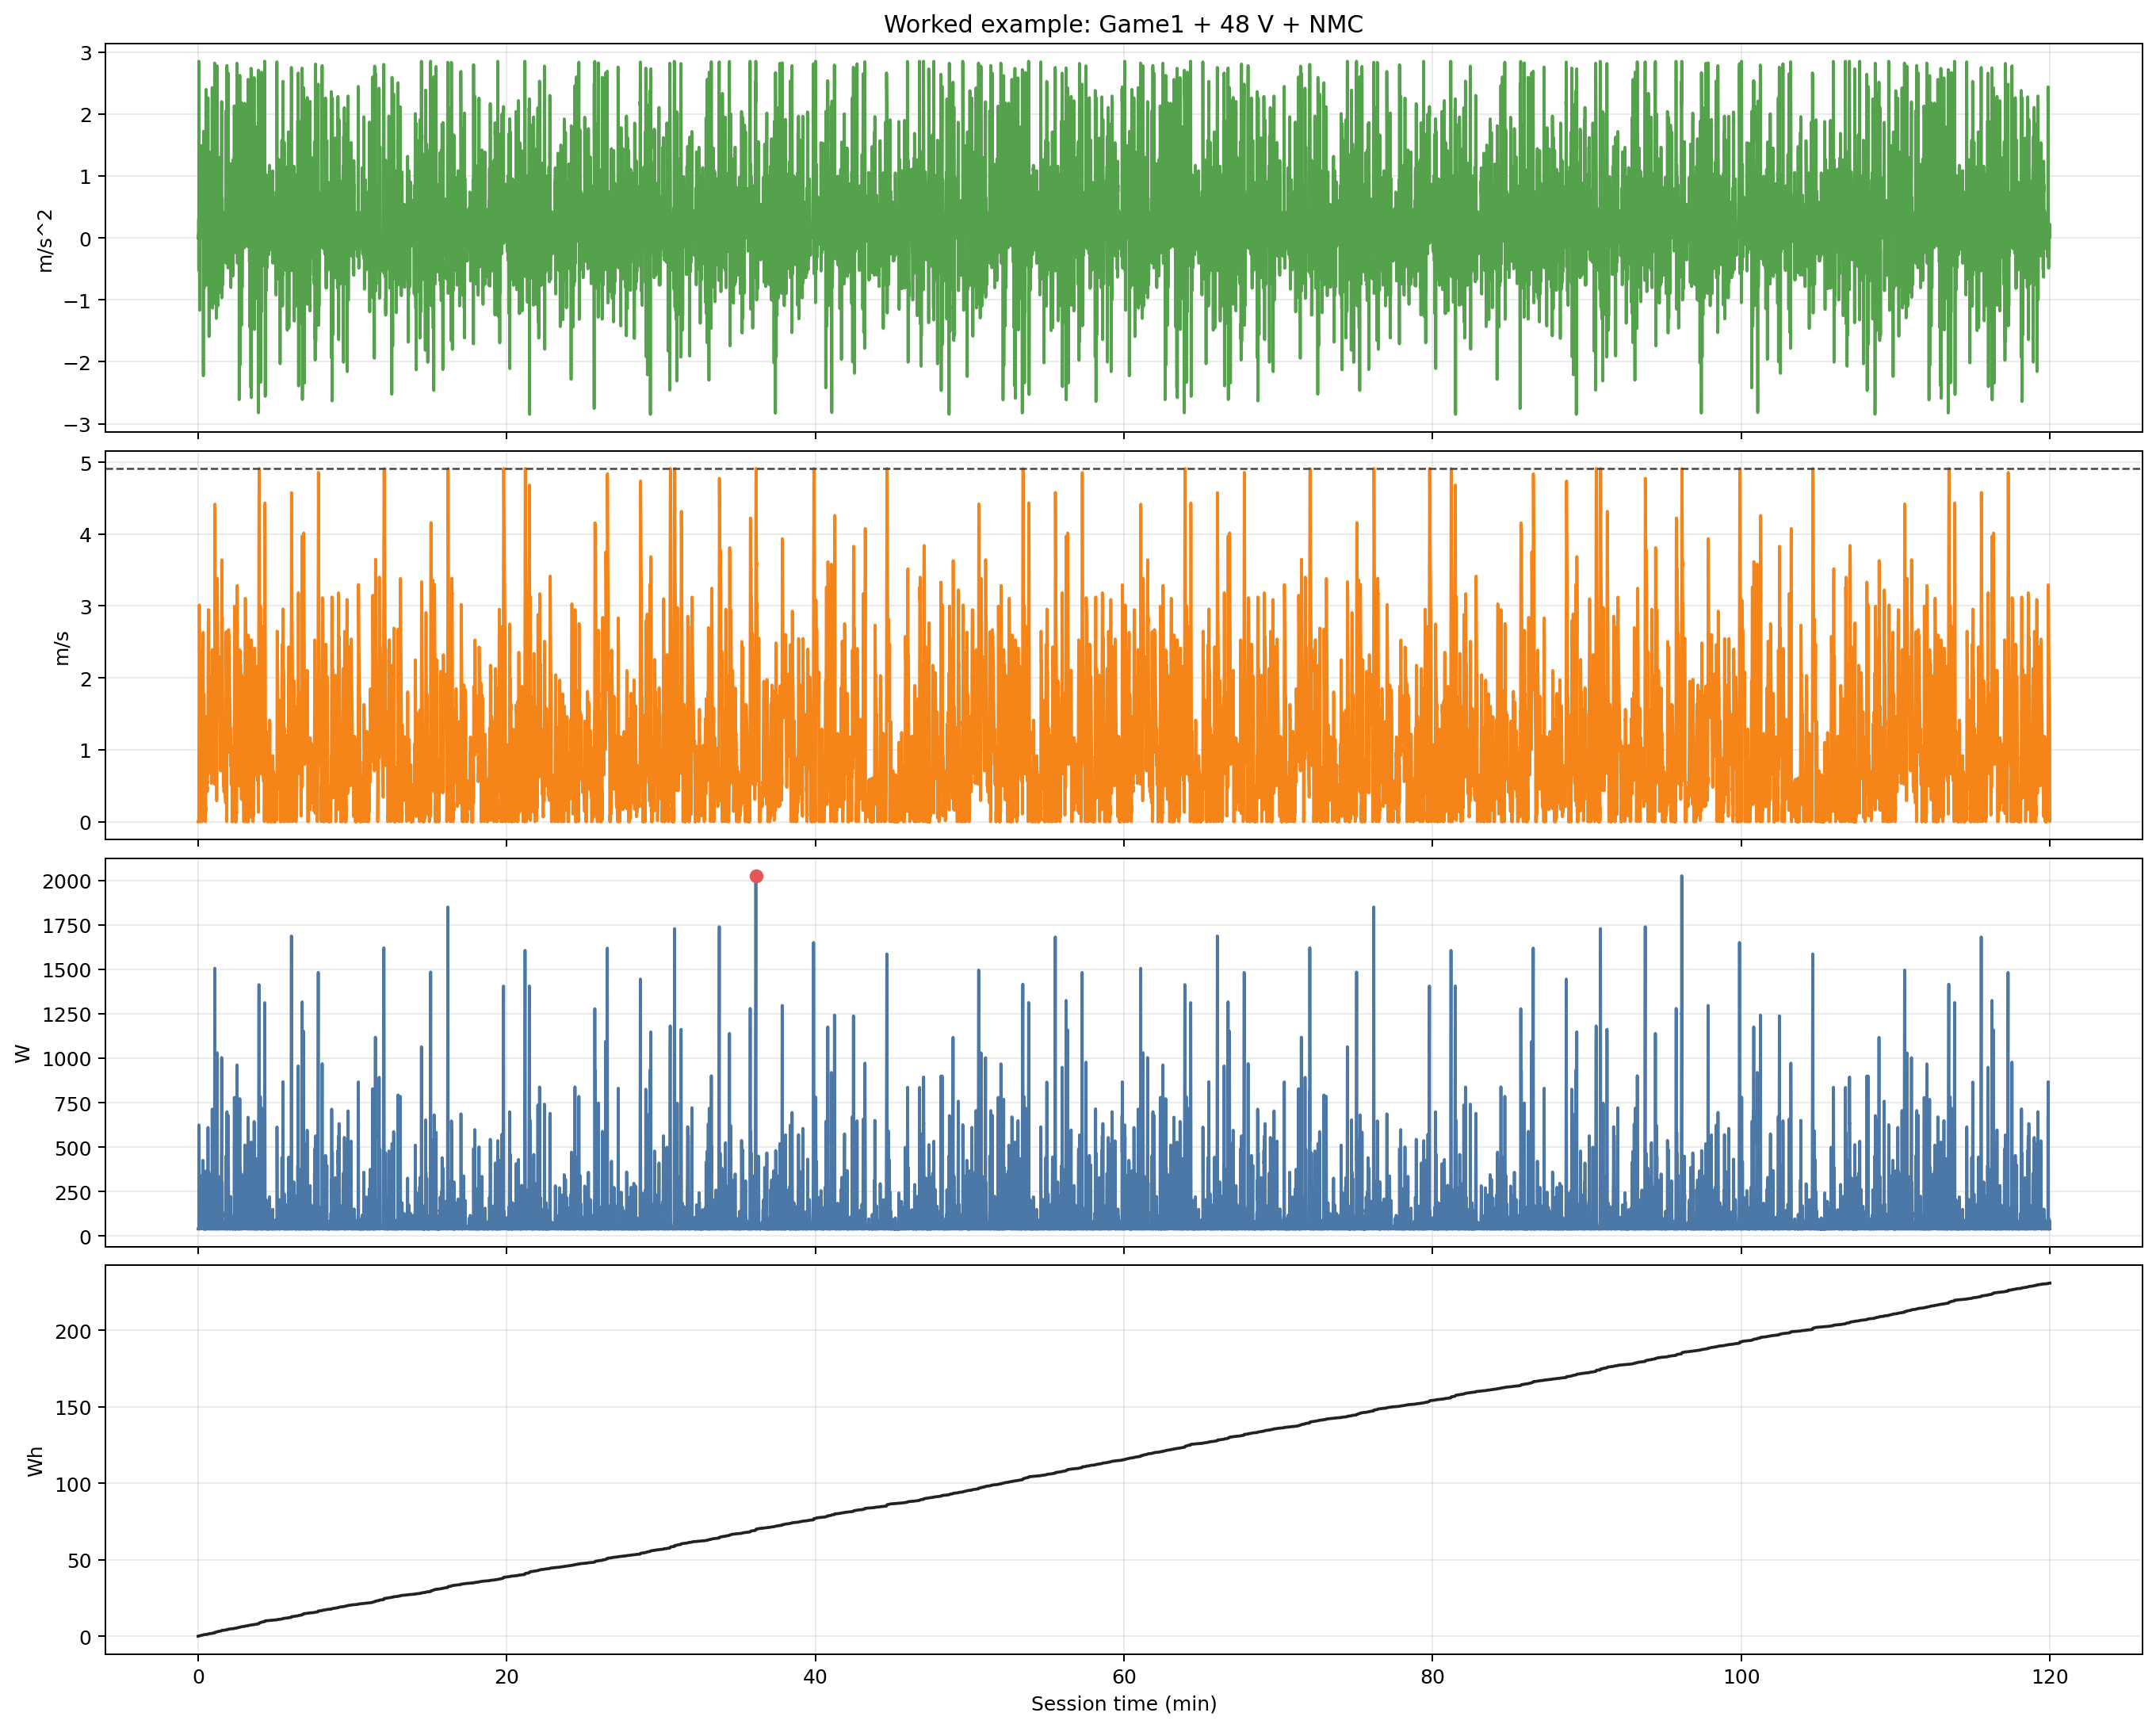
\includegraphics[width=\linewidth]{figures/worked_example.png}
  \caption{Worked-example time history. The final cumulative energy equals the usable gameplay energy in the official summary.}
\end{figure}

\section{Voltage And Chemistry Results}
For a fixed game, the cleaned gameplay energy is constant across voltage because the mechanical demand is unchanged. Higher voltage lowers pack current and required amp-hours. Chemistry changes nominal energy, mass, and C-rate checks.

\begin{figure}[H]
  \centering
  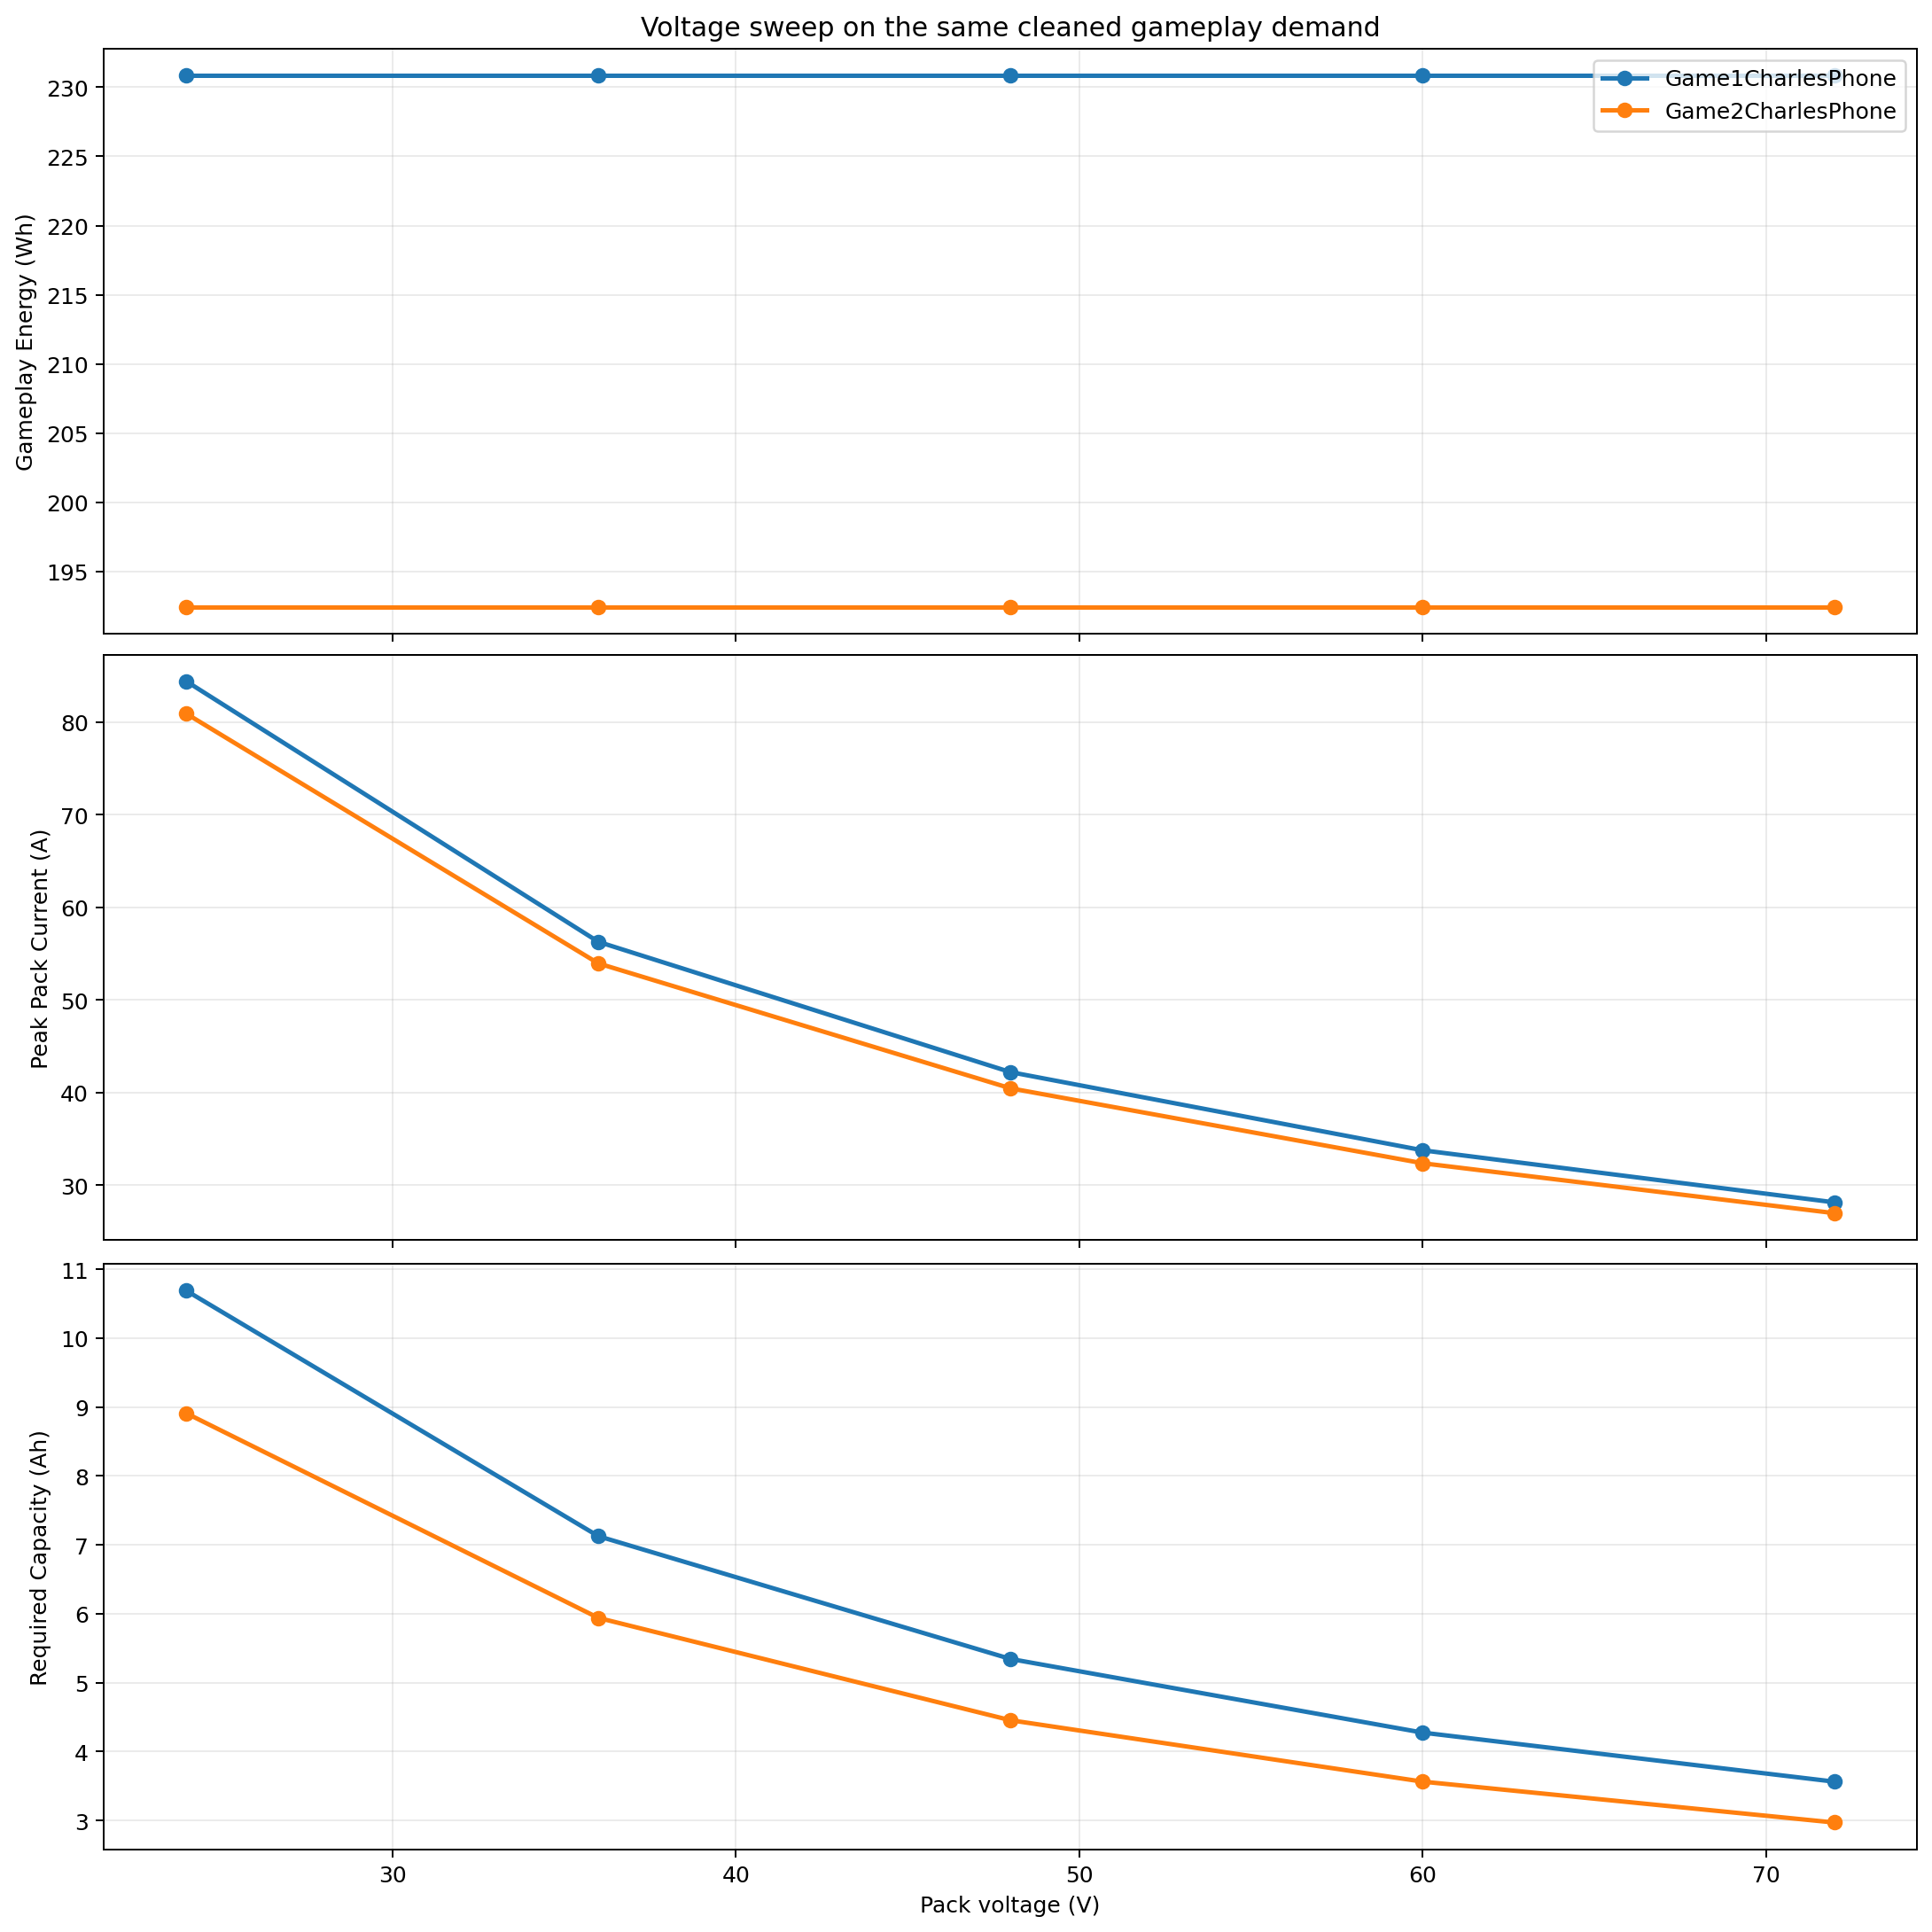
\includegraphics[width=\linewidth]{figures/voltage_sweep.png}
  \caption{Voltage sweep of the official gameplay-driven battery result.}
\end{figure}

\begin{figure}[H]
  \centering
  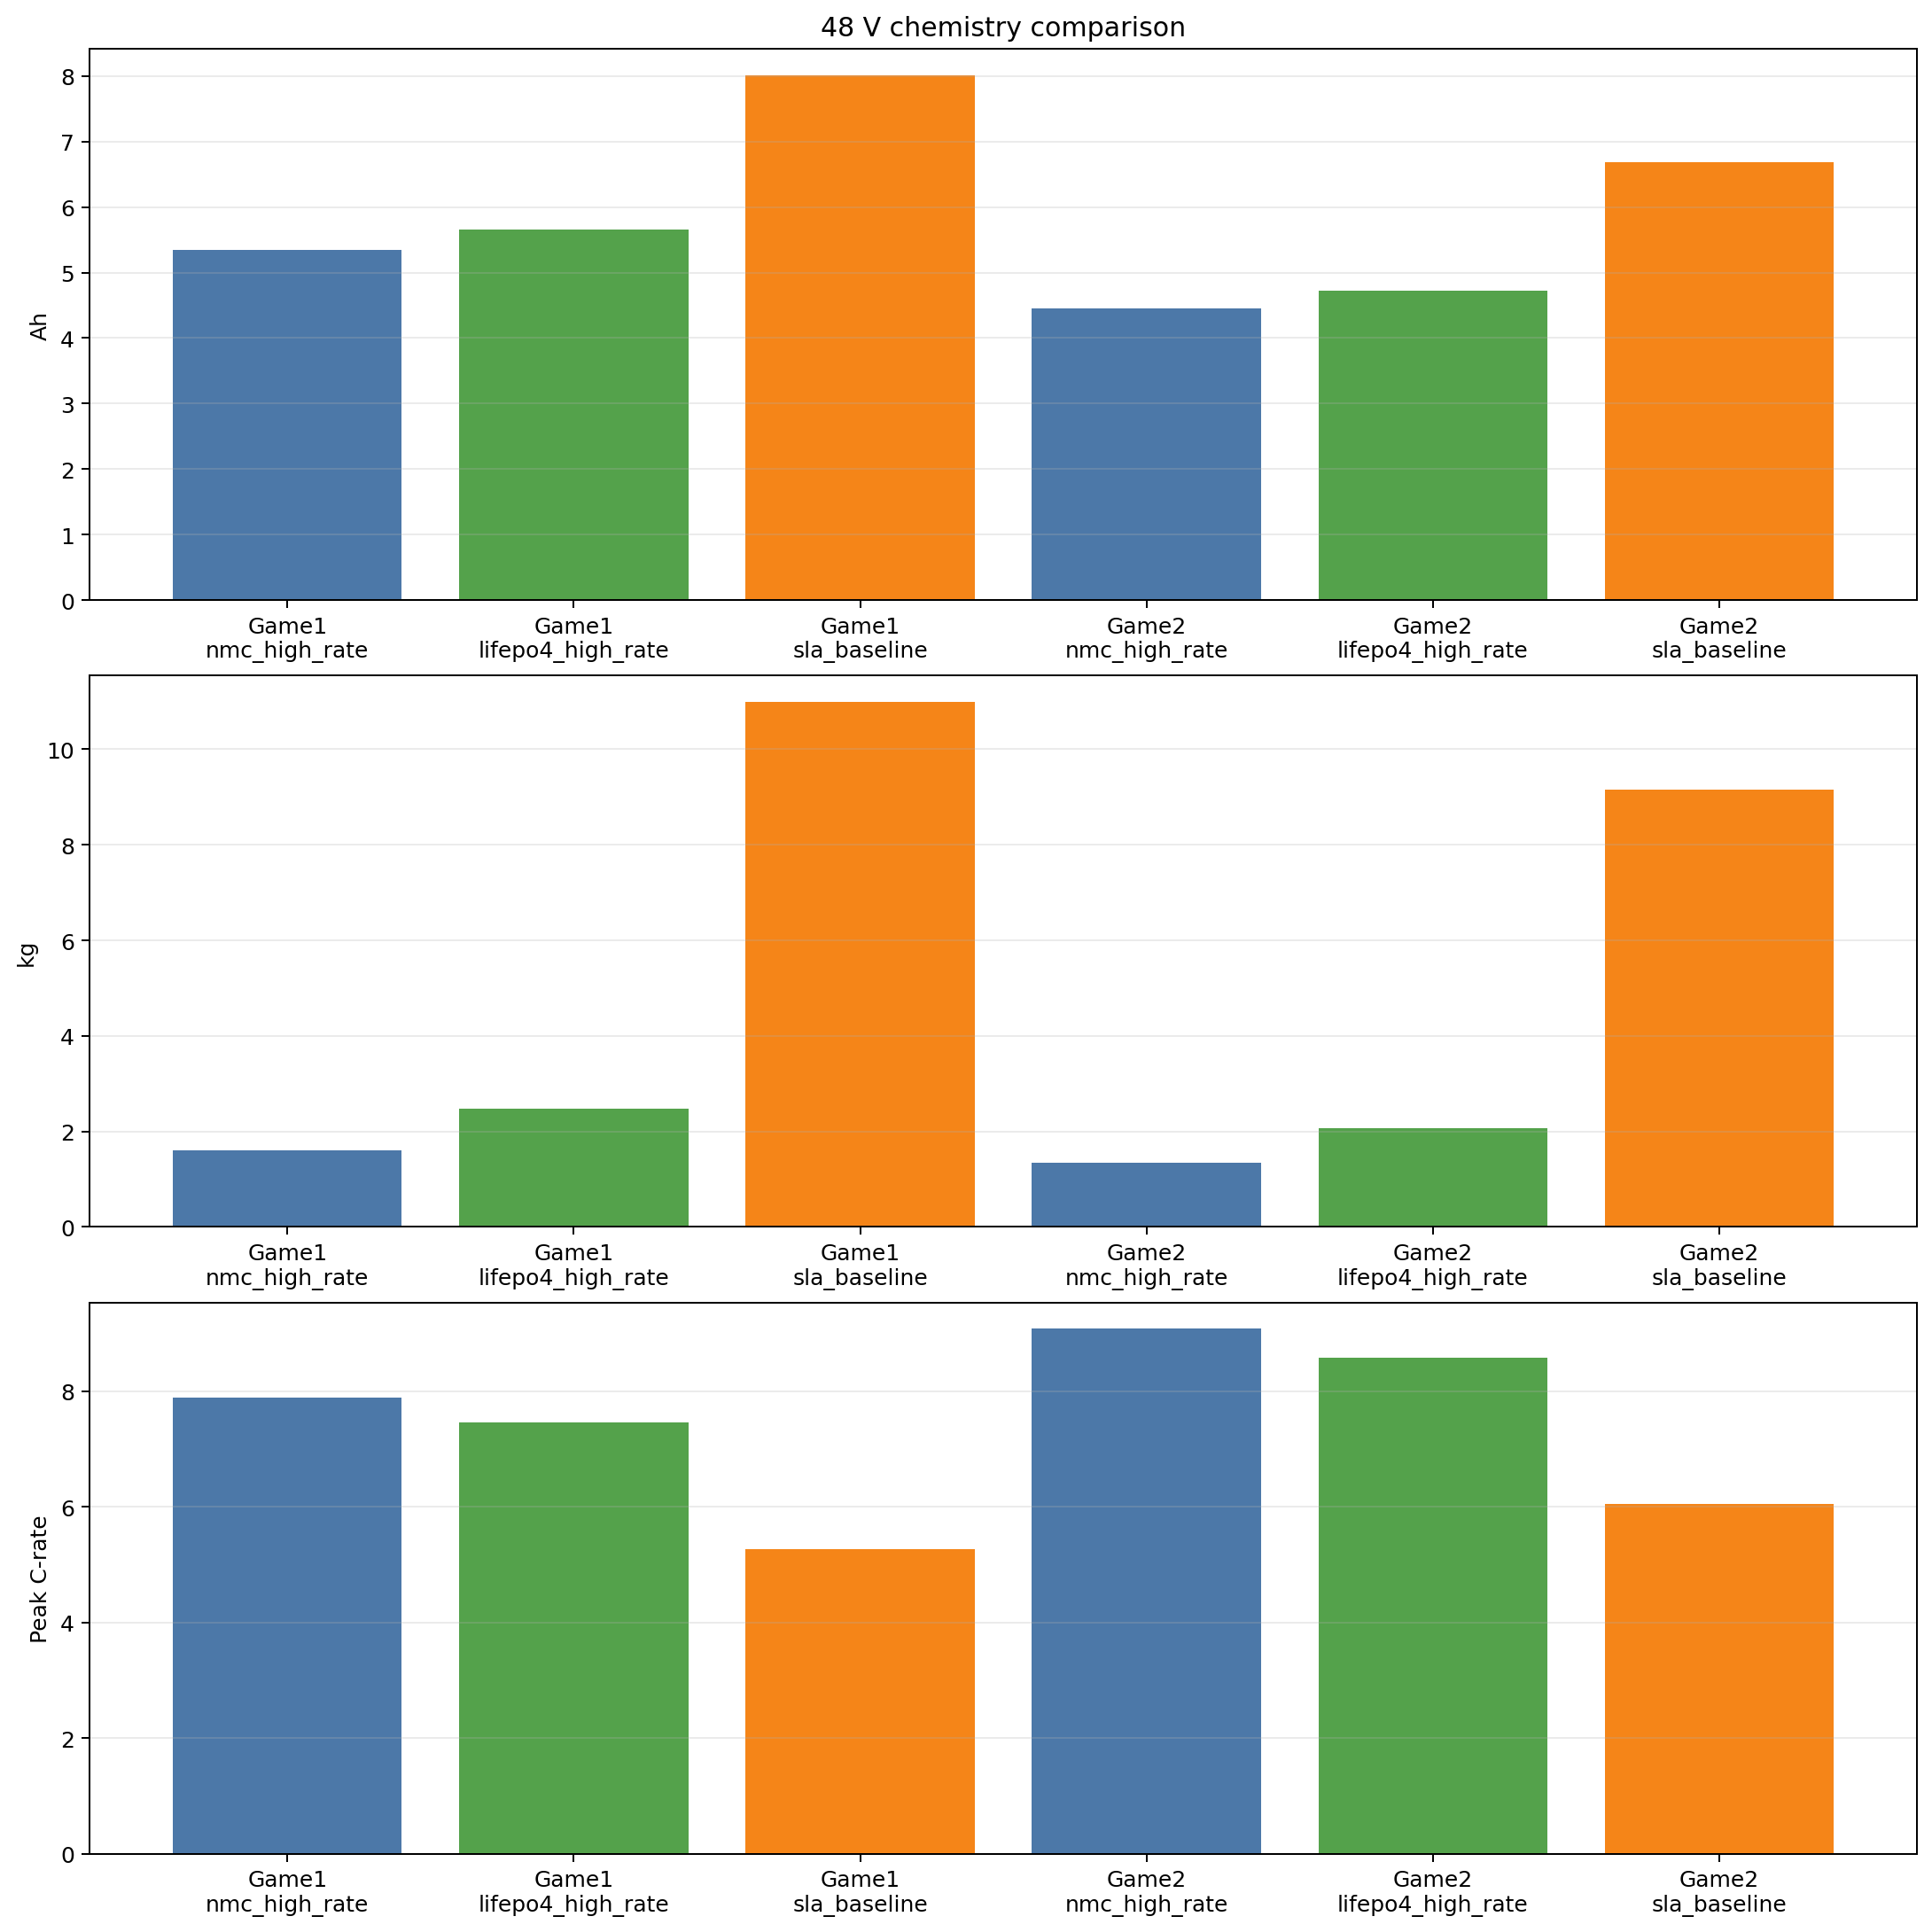
\includegraphics[width=\linewidth]{figures/chemistry_comparison_48v.png}
  \caption{Chemistry comparison at the 48 V design point.}
\end{figure}

\begin{longtable}{llllllllll}
\toprule
Game & Voltage (V) & Battery & Gameplay Energy (Wh) & Capacity (Ah) & Battery Mass (kg) & Peak Pack Current (A) & Peak C-Rate & Motor Peak Violation & Battery Peak Violation \\
\midrule
Game1CharlesPhone & 24 & nmc\_high\_rate & 230.85 & 10.69 & 1.60 & 84.39 & 7.90 & Yes & Yes \\
Game1CharlesPhone & 24 & lifepo4\_high\_rate & 230.85 & 11.32 & 2.47 & 84.39 & 7.46 & Yes & Yes \\
Game1CharlesPhone & 24 & sla\_baseline & 230.85 & 16.03 & 10.99 & 84.39 & 5.26 & Yes & Yes \\
Game1CharlesPhone & 36 & nmc\_high\_rate & 230.85 & 7.13 & 1.60 & 56.26 & 7.90 & Yes & Yes \\
Game1CharlesPhone & 36 & lifepo4\_high\_rate & 230.85 & 7.54 & 2.47 & 56.26 & 7.46 & Yes & Yes \\
Game1CharlesPhone & 36 & sla\_baseline & 230.85 & 10.69 & 10.99 & 56.26 & 5.26 & Yes & Yes \\
Game1CharlesPhone & 48 & nmc\_high\_rate & 230.85 & 5.34 & 1.60 & 42.20 & 7.90 & Yes & Yes \\
Game1CharlesPhone & 48 & lifepo4\_high\_rate & 230.85 & 5.66 & 2.47 & 42.20 & 7.46 & Yes & Yes \\
Game1CharlesPhone & 48 & sla\_baseline & 230.85 & 8.02 & 10.99 & 42.20 & 5.26 & Yes & Yes \\
Game1CharlesPhone & 60 & nmc\_high\_rate & 230.85 & 4.28 & 1.60 & 33.76 & 7.90 & Yes & Yes \\
Game1CharlesPhone & 60 & lifepo4\_high\_rate & 230.85 & 4.53 & 2.47 & 33.76 & 7.46 & Yes & Yes \\
Game1CharlesPhone & 60 & sla\_baseline & 230.85 & 6.41 & 10.99 & 33.76 & 5.26 & Yes & Yes \\
Game1CharlesPhone & 72 & nmc\_high\_rate & 230.85 & 3.56 & 1.60 & 28.13 & 7.90 & Yes & Yes \\
Game1CharlesPhone & 72 & lifepo4\_high\_rate & 230.85 & 3.77 & 2.47 & 28.13 & 7.46 & Yes & Yes \\
Game1CharlesPhone & 72 & sla\_baseline & 230.85 & 5.34 & 10.99 & 28.13 & 5.26 & Yes & Yes \\
Game2CharlesPhone & 24 & nmc\_high\_rate & 192.43 & 8.91 & 1.34 & 80.89 & 9.08 & Yes & Yes \\
Game2CharlesPhone & 24 & lifepo4\_high\_rate & 192.43 & 9.43 & 2.06 & 80.89 & 8.58 & Yes & Yes \\
Game2CharlesPhone & 24 & sla\_baseline & 192.43 & 13.36 & 9.16 & 80.89 & 6.05 & Yes & Yes \\
Game2CharlesPhone & 36 & nmc\_high\_rate & 192.43 & 5.94 & 1.34 & 53.93 & 9.08 & Yes & Yes \\
Game2CharlesPhone & 36 & lifepo4\_high\_rate & 192.43 & 6.29 & 2.06 & 53.93 & 8.58 & Yes & Yes \\
Game2CharlesPhone & 36 & sla\_baseline & 192.43 & 8.91 & 9.16 & 53.93 & 6.05 & Yes & Yes \\
Game2CharlesPhone & 48 & nmc\_high\_rate & 192.43 & 4.45 & 1.34 & 40.45 & 9.08 & Yes & Yes \\
Game2CharlesPhone & 48 & lifepo4\_high\_rate & 192.43 & 4.72 & 2.06 & 40.45 & 8.58 & Yes & Yes \\
Game2CharlesPhone & 48 & sla\_baseline & 192.43 & 6.68 & 9.16 & 40.45 & 6.05 & Yes & Yes \\
Game2CharlesPhone & 60 & nmc\_high\_rate & 192.43 & 3.56 & 1.34 & 32.36 & 9.08 & Yes & Yes \\
Game2CharlesPhone & 60 & lifepo4\_high\_rate & 192.43 & 3.77 & 2.06 & 32.36 & 8.58 & Yes & Yes \\
Game2CharlesPhone & 60 & sla\_baseline & 192.43 & 5.35 & 9.16 & 32.36 & 6.05 & Yes & Yes \\
Game2CharlesPhone & 72 & nmc\_high\_rate & 192.43 & 2.97 & 1.34 & 26.96 & 9.08 & Yes & Yes \\
Game2CharlesPhone & 72 & lifepo4\_high\_rate & 192.43 & 3.14 & 2.06 & 26.96 & 8.58 & Yes & Yes \\
Game2CharlesPhone & 72 & sla\_baseline & 192.43 & 4.45 & 9.16 & 26.96 & 6.05 & Yes & Yes \\
\bottomrule
\end{longtable}


\section{Verification Findings}
The main finding is that the current scenarios are not yet electrically comfortable under the present assumptions. The official summary still shows motor peak-current and battery peak C-rate violations.

That is a useful engineering result, not a reporting problem. It means the workflow is exposing the consequence of the current drivetrain and chemistry assumptions in a way a reviewer can check directly.

\begin{tabular}{lllllll}
\toprule
Game & Battery & Peak Motor Current (A) & Peak Pack Current (A) at 48 V & Peak C-Rate & Motor Peak Violation & Battery Peak Violation \\
\midrule
Game1CharlesPhone & nmc\_high\_rate & 47.99 & 42.20 & 7.90 & Yes & Yes \\
Game1CharlesPhone & lifepo4\_high\_rate & 47.99 & 42.20 & 7.46 & Yes & Yes \\
Game1CharlesPhone & sla\_baseline & 47.99 & 42.20 & 5.26 & Yes & Yes \\
Game2CharlesPhone & nmc\_high\_rate & 130.32 & 40.45 & 9.08 & Yes & Yes \\
Game2CharlesPhone & lifepo4\_high\_rate & 130.32 & 40.45 & 8.58 & Yes & Yes \\
Game2CharlesPhone & sla\_baseline & 130.32 & 40.45 & 6.05 & Yes & Yes \\
\bottomrule
\end{tabular}


\section{Assumptions Used}
The official assumptions used to generate this report are listed below.

\begin{longtable}{lll}
\toprule
Group & Parameter & Value \\
\midrule
Signal & resample\_hz & 100.0 \\
Signal & winsor\_percentile & 99.5 \\
Signal & lowpass\_cutoff\_hz & 0.5 \\
Signal & lowpass\_order & 4 \\
Signal & bias\_window\_s & 8.0 \\
Signal & linear\_lowpass\_cutoff\_hz & 1.25 \\
Signal & yaw\_lowpass\_cutoff\_hz & 1.5 \\
Signal & v\_max\_m\_s & 4.91744 \\
Signal & representative\_minutes & 60.0 \\
Signal & session\_hours & 2.0 \\
Signal & max\_realistic\_accel\_m\_s2 & 2.85 \\
Signal & impact\_accel\_threshold\_m\_s2 & 25.0 \\
Signal & impact\_jerk\_threshold\_m\_s3 & 120.0 \\
Signal & impact\_padding\_s & 0.35 \\
Signal & stationary\_accel\_threshold\_m\_s2 & 0.2 \\
Signal & stationary\_yaw\_rate\_threshold\_rad\_s & 0.2 \\
Signal & stationary\_hold\_s & 0.35 \\
Signal & velocity\_decay\_tau\_s & 8.0 \\
Vehicle & rider\_mass\_kg & 80.0 \\
Vehicle & chair\_mass\_without\_battery\_kg & 35.0 \\
Vehicle & system\_mass\_kg & 105.0 \\
Vehicle & pack\_voltage\_v & 48.0 \\
Vehicle & c\_rr & 0.002 \\
Vehicle & air\_density\_kg\_m3 & 1.225 \\
Vehicle & cd\_area\_m2 & 0.45 \\
Vehicle & grade\_rad & 0.0 \\
Vehicle & aux\_power\_w & 40.0 \\
Vehicle & equiv\_rotational\_inertia\_kg\_m2 & 0.0 \\
Vehicle & wheel\_rotational\_inertia\_kg\_m2\_per\_wheel & 0.2 \\
Vehicle & wheel\_track\_m & 0.68 \\
Vehicle & yaw\_inertia\_kg\_m2 & 10.0 \\
Vehicle & gravity\_m\_s2 & 9.80665 \\
Vehicle & initial\_battery\_mass\_guess\_kg & 5.0 \\
Vehicle & convergence\_tol\_kg & 0.05 \\
Vehicle & max\_iterations & 20 \\
Motor & name & 450w\_bldc\_planetary\_16to1 \\
Motor & motor\_mass\_kg & 3.5 \\
Motor & driven\_wheels & 2 \\
Motor & wheel\_radius\_m & 0.29845 \\
Motor & gear\_ratio & 16.0 \\
Motor & gear\_efficiency & 0.9 \\
Motor & torque\_constant\_nm\_per\_a & 0.12201365187713309 \\
Motor & continuous\_current\_a & 11.72 \\
Motor & peak\_current\_a & 35.24195804195804 \\
Motor & drivetrain\_efficiency & None \\
Motor & motor\_efficiency & 0.85 \\
Motor & rated\_torque\_nm & 1.43 \\
Motor & peak\_torque\_nm & 4.3 \\
Motor & rated\_speed\_rpm & 3000.0 \\
Battery nmc\_high\_rate & specific\_energy\_wh\_per\_kg / usable\_fraction / continuous\_c / peak\_c & 160.0, 0.9, 3.0, 5.0 \\
Battery lifepo4\_high\_rate & specific\_energy\_wh\_per\_kg / usable\_fraction / continuous\_c / peak\_c & 110.0, 0.85, 2.0, 3.0 \\
Battery sla\_baseline & specific\_energy\_wh\_per\_kg / usable\_fraction / continuous\_c / peak\_c & 35.0, 0.6, 0.5, 1.0 \\
\bottomrule
\end{longtable}


\appendix
\section{Official Plot Bundles}
For convenience, the report also includes the existing official summary plots generated by the battery-sizing script.

\begin{figure}[H]
  \centering
  
\includegraphics[width=\linewidth]{figures/Game1CharlesPhone_battery_sizing.png}
  \caption{Official battery-sizing plot bundle for Game 1.}
\end{figure}

\begin{figure}[H]
  \centering
  
\includegraphics[width=\linewidth]{figures/Game2CharlesPhone_battery_sizing.png}
  \caption{Official battery-sizing plot bundle for Game 2.}
\end{figure}

\end{document}
